% =============================================================================
%  Testing the failure model: probe results (research meeting, 19 Oct 2026)
%  Build: latexmk -pdf -outdir=tmp 2026-10-19-probe.tex   (figures come from ../results/)
% =============================================================================
\documentclass[aspectratio=169,11pt]{beamer}

\usepackage[T1]{fontenc}
\usepackage[utf8]{inputenc}
\usepackage[sfdefault]{plex-sans}
\usepackage{plex-mono}
\usepackage{microtype}
\usepackage[document]{ragged2e}
\usepackage{booktabs}
\usepackage{array}
\usepackage{graphicx}
\usepackage{tikz}
\usepackage{hyperref}
\graphicspath{{../results/}}

\hyphenpenalty=10000
\exhyphenpenalty=10000
\tolerance=3000

% ---------------------------------------------------------------------- palette
\definecolor{Ink}{HTML}{1A1C1E}
\definecolor{Body}{HTML}{303338}
\definecolor{Mute}{HTML}{74787E}
\definecolor{Rule}{HTML}{D3D6D9}
\definecolor{Panel}{HTML}{F2F3F4}
\definecolor{Accent}{HTML}{23405E}
\definecolor{Neg}{HTML}{8A3A2C}
\definecolor{PIblue}{HTML}{2A78D6}
\definecolor{FCorange}{HTML}{EB6834}
\definecolor{GAaqua}{HTML}{1BAF7A}

\setbeamercolor{background canvas}{bg=white}
\setbeamercolor{normal text}{fg=Body}
\setbeamercolor{frametitle}{fg=Ink}
\setbeamercolor{structure}{fg=Accent}
\setbeamerfont{normal text}{size=\fontsize{12}{15.5}}
\setbeamersize{text margin left=1.15cm,text margin right=1.15cm}

\setbeamertemplate{navigation symbols}{}
\setbeamertemplate{itemize item}{\color{Mute}\raise0.25ex\hbox{\rule{0.45ex}{0.45ex}}}
\setbeamertemplate{itemize subitem}{\color{Mute}\raise0.25ex\hbox{\rule{0.35ex}{0.35ex}}}

\setbeamerfont{frametitle}{series=\bfseries,size=\fontsize{16.5}{20}}
\setbeamertemplate{frametitle}{%
  \vspace{0.30cm}%
  \insertframetitle\par%
  \vspace{0.11cm}%
  {\color{Rule}\rule{\textwidth}{0.5pt}}%
}

\setbeamerfont{footline}{size=\fontsize{7.5}{9}}
\setbeamertemplate{footline}{%
  \leavevmode%
  \hbox{%
    \begin{beamercolorbox}[wd=\paperwidth,ht=0.26cm,dp=0.20cm,%
                           rightskip=1.15cm plus1fil]{footline}%
      \color{Mute}\hfill\insertframenumber
    \end{beamercolorbox}%
  }%
}

% ---------------------------------------------------------------------- helpers
\newcommand{\lbl}[1]{{\color{Mute}\fontsize{9.5}{12}\selectfont #1}\par}
\newcommand{\finding}[2]{%
  \noindent{\color{Accent}\fontsize{16}{19}\selectfont\bfseries #1}%
  \hspace{0.28em}{\color{Body}\fontsize{10.5}{13.5}\selectfont #2}\par}
\newcommand{\fnote}[1]{{\color{Mute}\fontsize{8.5}{11}\selectfont #1\par}}
\newcommand{\code}[1]{{\ttfamily\fontsize{8.6}{11.4}\selectfont #1}}
\newcommand{\sw}[1]{\tikz[baseline=-0.6ex]\fill[#1] (0,-0.09) rectangle (0.22,0.13);}

\begin{document}

% == 1 == Title ================================================================
\begin{frame}[plain]
  \vspace{1.05cm}
  {\color{Ink}\fontsize{25}{30}\selectfont\bfseries
    Testing the failure model:\\[0.05cm]
    a probe on two public datasets\par}
  \vspace{0.54cm}
  {\color{Body}\fontsize{13}{17}\selectfont
    PageIndex matched full context where we predicted failure. What this changes.\par}
  \vspace{0.90cm}
  {\color{Rule}\rule{0.42\textwidth}{0.5pt}\par}
  \vspace{0.36cm}
  {\color{Ink}\fontsize{12.5}{16}\selectfont Aniruddha Chattopadhyay\par}
  \vspace{0.12cm}
  {\color{Mute}\fontsize{10.5}{14}\selectfont Research meeting with Prof.\ Kaushik Roy and Ash \hspace{0.5em}·\hspace{0.5em} 19 October 2026\par}
\end{frame}

% == 2 == The probe in one slide ==============================================
\begin{frame}{The probe in one slide}
  \vspace{0.25cm}
  \begin{columns}[T,onlytextwidth]
    \begin{column}{0.52\textwidth}
      \lbl{Accuracy: PageIndex against full context, same model}
      \vspace{0.12cm}
      \finding{0.68 vs 0.67}{F1, DesignQA Compilation: all rules about a topic (30 questions)}
      \vspace{0.10cm}
      \finding{0.98 vs 0.98}{F1, DesignQA Retrieval: one rule by its number (20 questions)}
      \vspace{0.10cm}
      \finding{13 vs 12}{correct, LongMemEval: questions about a dated chat history (15 questions)}
    \end{column}
    \begin{column}{0.42\textwidth}
      \lbl{Input tokens for each Compilation question}
      \vspace{0.12cm}
      \finding{172k}{PageIndex}
      \vspace{0.10cm}
      \finding{81k}{full context: the whole document}
      \vspace{0.30cm}
      \lbl{Main message}
      \vspace{0.08cm}
      {\fontsize{11.5}{15}\selectfont\color{Ink}\bfseries Our predictions failed where we expected PageIndex to fail. PageIndex reads widely: it keeps its accuracy and pays with tokens.\par}
    \end{column}
  \end{columns}
\end{frame}

% == 3 == Setup and predictions ================================================
\begin{frame}{We wrote the predictions before the runs}
  \vspace{0.20cm}
  \begin{columns}[T,onlytextwidth]
    \begin{column}{0.45\textwidth}
      \lbl{Data and systems}
      \vspace{0.06cm}
      {\fontsize{9.5}{12.2}\selectfont
      \begin{itemize}\setlength{\itemsep}{2pt}
        \item \textbf{DesignQA:} one 140-page Formula SAE rules PDF with 588 bookmarks. Official F1, no judge.
        \item \textbf{LongMemEval S:} one PDF for each question, about 48 dated chat sessions (165 pages). Official judge.
        \item \textbf{Three systems}, same model and instructions: \sw{PIblue} PageIndex 0.4.1 (local, Flash index), \sw{FCorange} full context, and a keyword agent (BM25 search and page reading).
      \end{itemize}}
    \end{column}
    \begin{column}{0.51\textwidth}
      \lbl{Key predictions, written on 16 October before any run}
      \vspace{0.10cm}
      {\fontsize{9.5}{12.3}\selectfont
      \begin{tabular}{@{}p{0.55cm}p{3.9cm}p{1.75cm}@{}}
        \toprule
        \textbf{P1} & Retrieval: PageIndex equals full context & A1, A2 true \\[3pt]
        \textbf{P2} & Compilation: PageIndex at least 0.10 F1 below full context & A2 false \\[3pt]
        \textbf{P7} & Multi-session, update and temporal questions: PageIndex wrong more often & A2, A4 false \\
        \bottomrule
      \end{tabular}\par}
      \vspace{0.18cm}
      \fnote{The rule in the file: if P2 and P7 both fail, the model is wrong for these datasets.}
    \end{column}
  \end{columns}
\end{frame}

% == 4 == DesignQA =============================================================
\begin{frame}{DesignQA: the same accuracy at twice the tokens}
  \vspace{0.05cm}
  \centering
  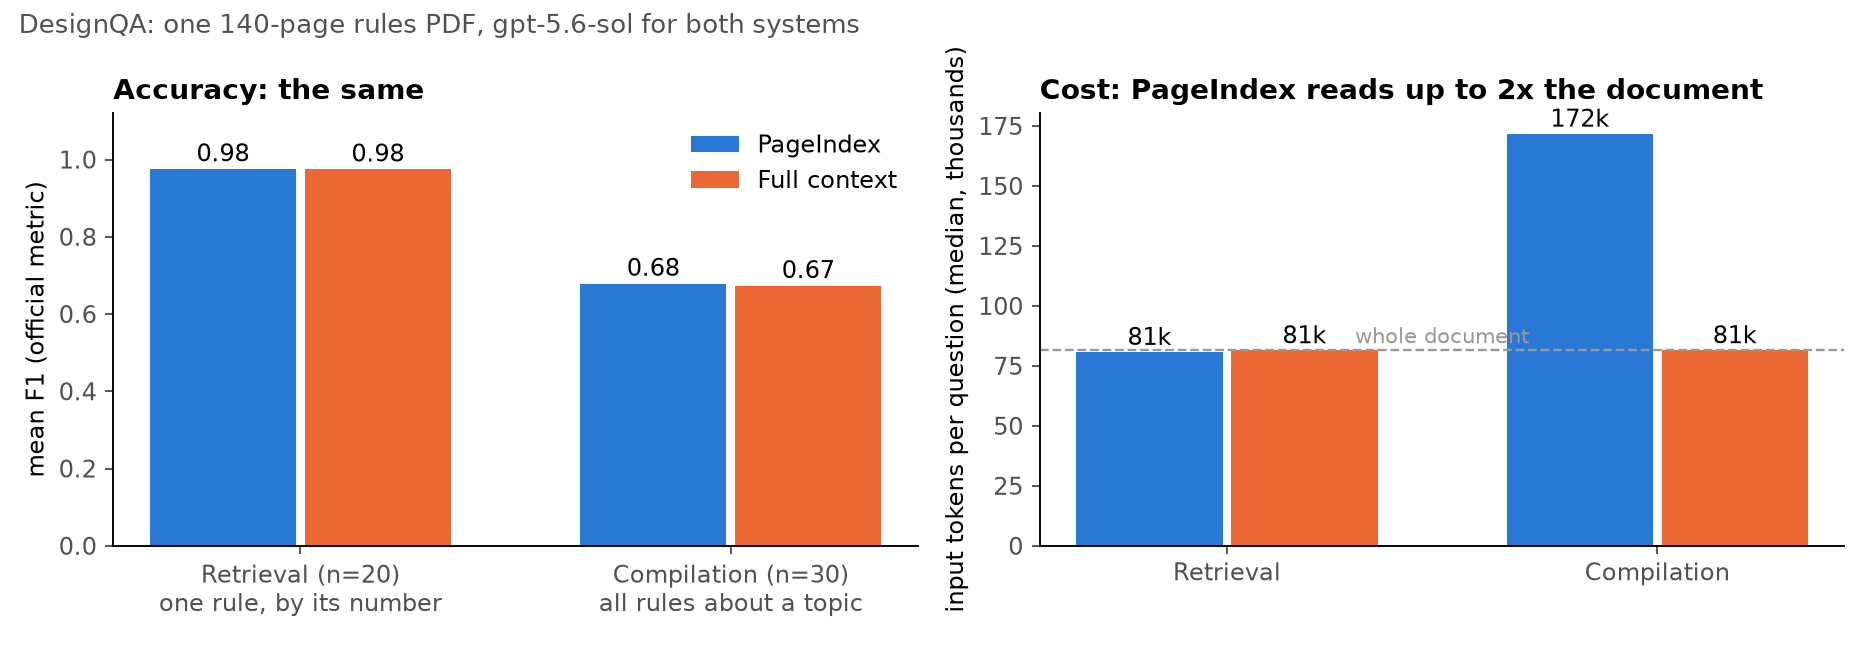
\includegraphics[width=\textwidth]{probe_fig1_designqa.png}\par
  \vspace{0.05cm}
  \fnote{gpt-5.6-sol for both systems. On Compilation, PageIndex read a median of 19 pages, including 80\% of the pages with gold rules. Cost for each Compilation question: PageIndex \$0.36; full context about \$0.05 with a prompt cache.}
\end{frame}

% == 5 == LongMemEval ===========================================================
\begin{frame}{LongMemEval: PageIndex was not worse}
  \vspace{0.20cm}
  \begin{columns}[T,onlytextwidth]
    \begin{column}{0.53\textwidth}
      \lbl{15 questions, 3 of each type}
      \vspace{0.10cm}
      {\fontsize{9.5}{12.5}\selectfont\setlength{\tabcolsep}{4pt}
      \begin{tabular}{@{}lrrr@{}}
        \toprule
        & PageIndex & Full & Keyword \\
        \midrule
        Correct (of 15) & \textbf{13} & 12 & 12 \\
        Tokens (median) & 42k & 118k & 5k \\
        Cost per question & \$0.006 & \$0.024 & \$0.001 \\
        \bottomrule
      \end{tabular}\par}
      \vspace{0.25cm}
      {\fontsize{10}{13}\selectfont PageIndex read all the answer sessions in 10 of 15 questions. All three systems missed the same temporal question.\par}
    \end{column}
    \begin{column}{0.43\textwidth}
      \lbl{Why: the labels name the key}
      \vspace{0.10cm}
      {\setlength{\fboxsep}{7pt}\colorbox{Panel}{\parbox{0.93\linewidth}{\fontsize{10}{13.5}\selectfont
        \textbf{Question:} ``What size is my new Samsung TV?'' \hfill {\color{Mute}gold: 55-inch}\par
        \vspace{0.12cm}
        \textbf{Label of the answer session:} ``\dots\ The user describes organizing cables on a \textbf{Samsung 55-inch} 4K TV \dots''\par}}}\par
      \vspace{0.20cm}
      {\fontsize{10}{13}\selectfont A chat session has one topic, so a 150-word summary names its main facts.\par}
    \end{column}
  \end{columns}
  \vspace{0.25cm}
  \fnote{gpt-5.6-luna for all three systems, to save budget. Judge: gpt-4o-2024-08-06 with the official LongMemEval prompts.}
\end{frame}

% == 6 == Scorecard ============================================================
\begin{frame}{Scorecard of the predictions}
  \vspace{0.02cm}
  {\fontsize{9}{11.2}\selectfont
  \renewcommand{\arraystretch}{1.0}\setlength{\tabcolsep}{4pt}
  \begin{tabular}{@{}p{0.6cm}p{7.3cm}p{2.3cm}p{2.6cm}@{}}
    \toprule
    & Prediction & Result & Evidence \\
    \midrule
    P1 & Retrieval: PageIndex within 0.05 F1 of full & Held & 0.976 vs 0.975 \\
    P2 & Compilation: PageIndex $\geq$ 0.10 F1 below full & \textcolor{Neg}{\textbf{False}} & 0.679 vs 0.673 \\
    P3 & Compilation: F1 falls as the gold list grows & Held, near zero & Spearman $-0.08$ \\
    P4 & Compilation: $<$ half of the gold pages read & \textcolor{Neg}{\textbf{False}} & median 0.80 \\
    P5 & Compilation: the keyword agent beats PageIndex & Not tested & budget \\
    P6 & Single-session-user: at most one more error & Held & 0 vs 0 errors \\
    P7 & Multi-session, update, temporal: PageIndex worse & \textcolor{Neg}{\textbf{False}} & 1 vs 2 errors \\
    P8 & Those errors come from unread answer sessions & Not supported & error had both \\
    P9 & Abstention: PageIndex reads more pages & Held & 11.0 vs 5.3 pages \\
    P10 & DesignQA labels hold $>$ 15\% of the PDF words & Held & 55\% \\
    \bottomrule
  \end{tabular}\par}
  \vspace{0.14cm}
  {\fontsize{11}{14}\selectfont\color{Ink}\bfseries P2 and P7 are both false. By our own rule, the model is wrong for single documents of about 150 pages.\par}
\end{frame}

% == 7 == Revised model =========================================================
\begin{frame}{Revised model: evidence out of reach}
  \vspace{0.20cm}
  \begin{columns}[T,onlytextwidth]
    \begin{column}{0.50\textwidth}
      {\fontsize{10}{13}\selectfont
      \textbf{1. Dense sections.} The labels cannot name the facts.\par
      {\color{Mute}CLEVRER pilot: the labels held 6.4\% of the numbers of a run. PageIndex 87.5\% against 95.2\%.}\par
      \vspace{0.16cm}
      \textbf{2. Large corpora.} The agent cannot read the spread, or the tree does not fit.\par
      {\color{Mute}RIT-RAG (IBM, Oct 2026): 66.7--75.3\% on FinanceBench with 364 filings; no run on 2.84 million pages.}\par
      \vspace{0.16cm}
      \textbf{Otherwise, PageIndex pays with tokens.} Spread alone does not cause errors.\par}
    \end{column}
    \begin{column}{0.46\textwidth}
      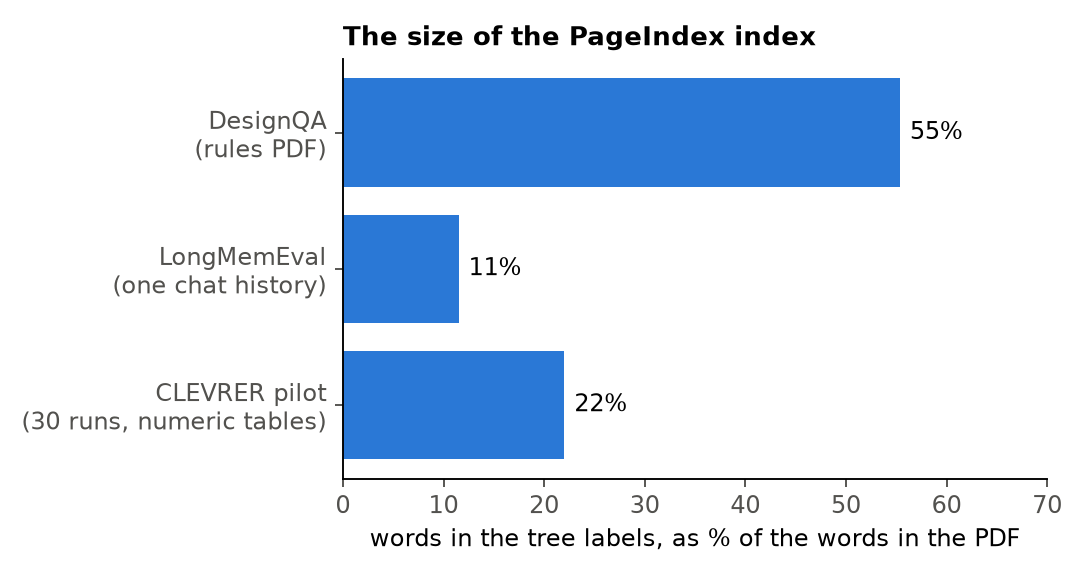
\includegraphics[width=\linewidth]{probe_fig3_labels.png}\par
    \end{column}
  \end{columns}
\end{frame}

% == 8 == Next =================================================================
\begin{frame}{Next tests and decisions}
  \vspace{0.20cm}
  \begin{columns}[T,onlytextwidth]
    \begin{column}{0.53\textwidth}
      \lbl{Next tests: where the revised model predicts failure}
      \vspace{0.06cm}
      {\fontsize{10}{13}\selectfont
      \begin{enumerate}\setlength{\itemsep}{3pt}
        \item \textbf{Dense records:} a maintenance log from the AssetOpsBench work orders and sensor tables, with exact answers.
        \item \textbf{Scale:} LongMemEval M, about 500 sessions and 1.5 million tokens for each question. Full context does not fit.
        \item \textbf{Baseline:} keep the keyword agent. On LongMemEval it matched PageIndex at one fifth of the cost.
      \end{enumerate}}
    \end{column}
    \begin{column}{0.43\textwidth}
      \lbl{Decisions}
      \vspace{0.06cm}
      {\fontsize{10}{13}\selectfont
      \begin{enumerate}\setlength{\itemsep}{3pt}
        \item Do we accept the revised model?
        \item Budget for the next tests: about \$10--15 with gpt-5.6-luna. The probe cost \$31.94.
        \item A separate OpenRouter key for this project. The current key is shared.
      \end{enumerate}}
    \end{column}
  \end{columns}
\end{frame}

% == 9 == Backup: limits =======================================================
\begin{frame}{Backup: the limits of this probe}
  \vspace{0.20cm}
  {\fontsize{10.5}{14}\selectfont
  \begin{itemize}\setlength{\itemsep}{4pt}
    \item Small samples: 15 LongMemEval questions, and one run for each question.
    \item PageIndex varies from run to run. One Compilation question got F1 0.11 in a check run and 0.69 in the main run.
    \item Two chat models: gpt-5.6-sol for DesignQA, and gpt-5.6-luna for LongMemEval.
    \item The keyword agent did not run on DesignQA.
    \item The Compilation gold follows a fixed rule (sub-rules and cited rules) that the question does not state. So both systems stop at about 0.67, and this limit can hide differences.
    \item The full-context runs on DesignQA did not use the prompt cache in parallel. Sequential calls cost \$0.033 instead of \$0.33.
  \end{itemize}}
\end{frame}

\end{document}
